\chapter{Theoretical introduction\label{sec:intro}}

%Standard Model
% - What does it consist of (particles, interactions, gauge fields)
% - Description of Higgs mechanism and its significance
% - Examples of SM limitations (DM, gravity, Higgs loop corrections...)

%Supersymmetry
% - What is supersymmetry, what SM problems does it address
% - 2HDM, NMSSM: Motivations
% - 

\section{The Standard Model\label{sec:SM}}

This chapter presents an overview of some of the main theoretical developments leading up to the Standard Model of fundamental physics, followed by an overview of the theory of supersymmetry and how it addresses some of the Standard Model's deficiencies.

\subsection{A little background\label{sec:SM-history}}

Classical physics differentiates clearly between matter particles, which behave as localized objects, and radiation, which behaves as a wave. However, when physicists explored phenomena at the subatomic scale, the classical picture was found to be incorrect. The discovery of phenomena such as the photoelectric effect and the Compton effect, which point to the quantization of radiation, challenged classical assumptions about the wave behavior of light. Similarly, observations of diffraction behavior in electron beams revealed that beams of electrons can in fact behave not only like pointlike bodies but also like light waves~\cite{MessiahPhysics}. The quest to understand this wave-particle duality led to the development of quantum mechanics to explain physical phenomena at the microscopic scale.

In quantum mechanics, the physical state of a particle or system of particles is characterized by a wavefunction. Measurable properties of particles, such as position and momentum, can all be derived from the wavefunction. The wavelike behavior of particles at the subatomic scale is reflected in the plane-wave wavefunction for free particles, and the bound-state wavefunctions that are related to standing waves, with discrete (quantized) energy levels available to the particles in the bound system.

Quantum field theory developed from the need to describe the dynamics of relativistic elementary particles, for which nonrelativistic quantum mechanics is insufficient. For instance, consider the Klein-Gordon equation

\begin{equation}
(\partial^{\mu}\partial_{\mu} + m^{2})\phi = 0\newline
\label{eq:KG}
\end{equation}
which is the relativistic wave equation of motion for relativistic spin-0 particles. The plane-wave solutions to the Klein-Gordon equation have positive and negative energies, which correspond to particles with positive and negative probability densities. The latter concept is clearly nonphysical, but in the formalism of QFT, the negative-energy solutions acquire a physical interpretation\cite{PeskinSchroederPhysics,ThomsonPhysics}. For each particle, there exists an antiparticle with identical mass and spin but opposite charge. The solution $\phi$ to the Klein-Gordon equation is not a single-particle wavefunction, but rather a scalar field, whose excitations correspond to the creation and annihilation of particles and antiparticles. The antiparticle corresponds to the negative-energy portion of the solution to the Klein-Gordon equation.

The same logic, applied to Dirac equation of motion for spin-$\frac{1}{2}$ particles,

\begin{equation}
(i\gamma^{\mu}\partial_{\mu} - m)\psi = 0
\label{eq:Dirac}
\end{equation}
led to the prediction of the existence of the positron, the antiparticle of the electron. Experimental support for this theory first came with the discovery of the positron in cloud-chamber studies of cosmic rays~\cite{BettiniPhysics}, confirming the existence of antiparticles and validating the description of particle physics with quantum field theory.

Particles interact via four fundamental forces: the strong force, electromagnetism, the weak force, and gravity. So far, the first three types of interactions have been successfully described by quantum field theories. The dynamics and interactions of fields are derived from the Lagrangian density $\mathcal{L}$, which is the quantum field theory analogue of the classical Lagrangian $L$ that is defined as the difference between the total kinetic and potential energy of a system of particles. While $L$ is a function of the coordinates and momenta of all particles in a system, $\mathcal{L}$ is a function of fields and their spacetime derivatives.

By Noether's theorem, the invariance of $\mathcal{L}$ under continuous transformations of the fields implies the conservation of a current. Such transformations that leave $\mathcal{L}$ invariant are called symmetry transformations, and can be expressed in terms of the generators of a symmetry group. Each fundamental interaction is governed by the invariance of $\mathcal{L}$ under local (i.e., spacetime-dependent) phase transformations known as gauge transformations, and transitions between states are constrained by the quantum numbers and conserved current associated with that interaction.

The invariance requirement for $\mathcal{L}$ necessitates the transformation of spacetime derivatives $\partial_{\mu}$ in the Lagrangian via the generators of the symmetry group. These generators correspond to gauge fields whose excitations are the gauge bosons that mediate the fundamental interaction. As a simple illustration, in the QED Lagrangian which obeys the symmetry of the unitary group U(1):

\begin{eqnarray}
\mathcal{L}_{QED} &=& \bar{\psi}(i\gamma^{\mu}D_{\mu} - m)\psi -\frac{1}{4}F^{\mu\nu}F_{\mu\nu} \nonumber \\
    &=& \bar{\psi}(i\gamma^{\mu}D_{\mu} - m)\psi -\frac{1}{4}(\partial^{\mu}A^{\nu} - \partial^{\nu}A^{\mu})(\partial_{\mu}A_{\nu} - \partial_{\nu}A_{\mu})
\label{eq:QEDLagrangian}
\end{eqnarray}

the gauge covariant derivative $D_{\mu}$ is given by:

\begin{equation}
D_{\mu} = \partial_{\mu} + ieA_{\mu}
\label{eq:covariant-derivative}
\end{equation}
where $A_{\mu}$ is the field corresponding to the photon, the gauge boson of the QED theory. Once $A_{\mu}$ is introduced and the gauge covariant derivative is thus defined, $\mathcal{L}$ is invariant under all U(1) transformations $\psi \rightarrow \psi' = e^{i\chi(x)}\psi$.

Developing field theory descriptions for the fundamental forces has led to predictions of the existence of many new particles. Over the decades, high-energy physics experiments have confirmed the existence of these particles. The Standard Model is the quantum field theory that provides the most successful description to date of all experimentally observed fundamental particles and their interactions. The following section presents a summary of the current state of the Standard Model and its categorization of all known fundamental particles.

\subsection{Particles of the Standard Model\label{sec:SM-particles}}

A tabular display of all experimentally observed fundamental particles is shown in Figure~\ref{fig:StandardModelTable}.

\begin{figure}
   \begin{center}
      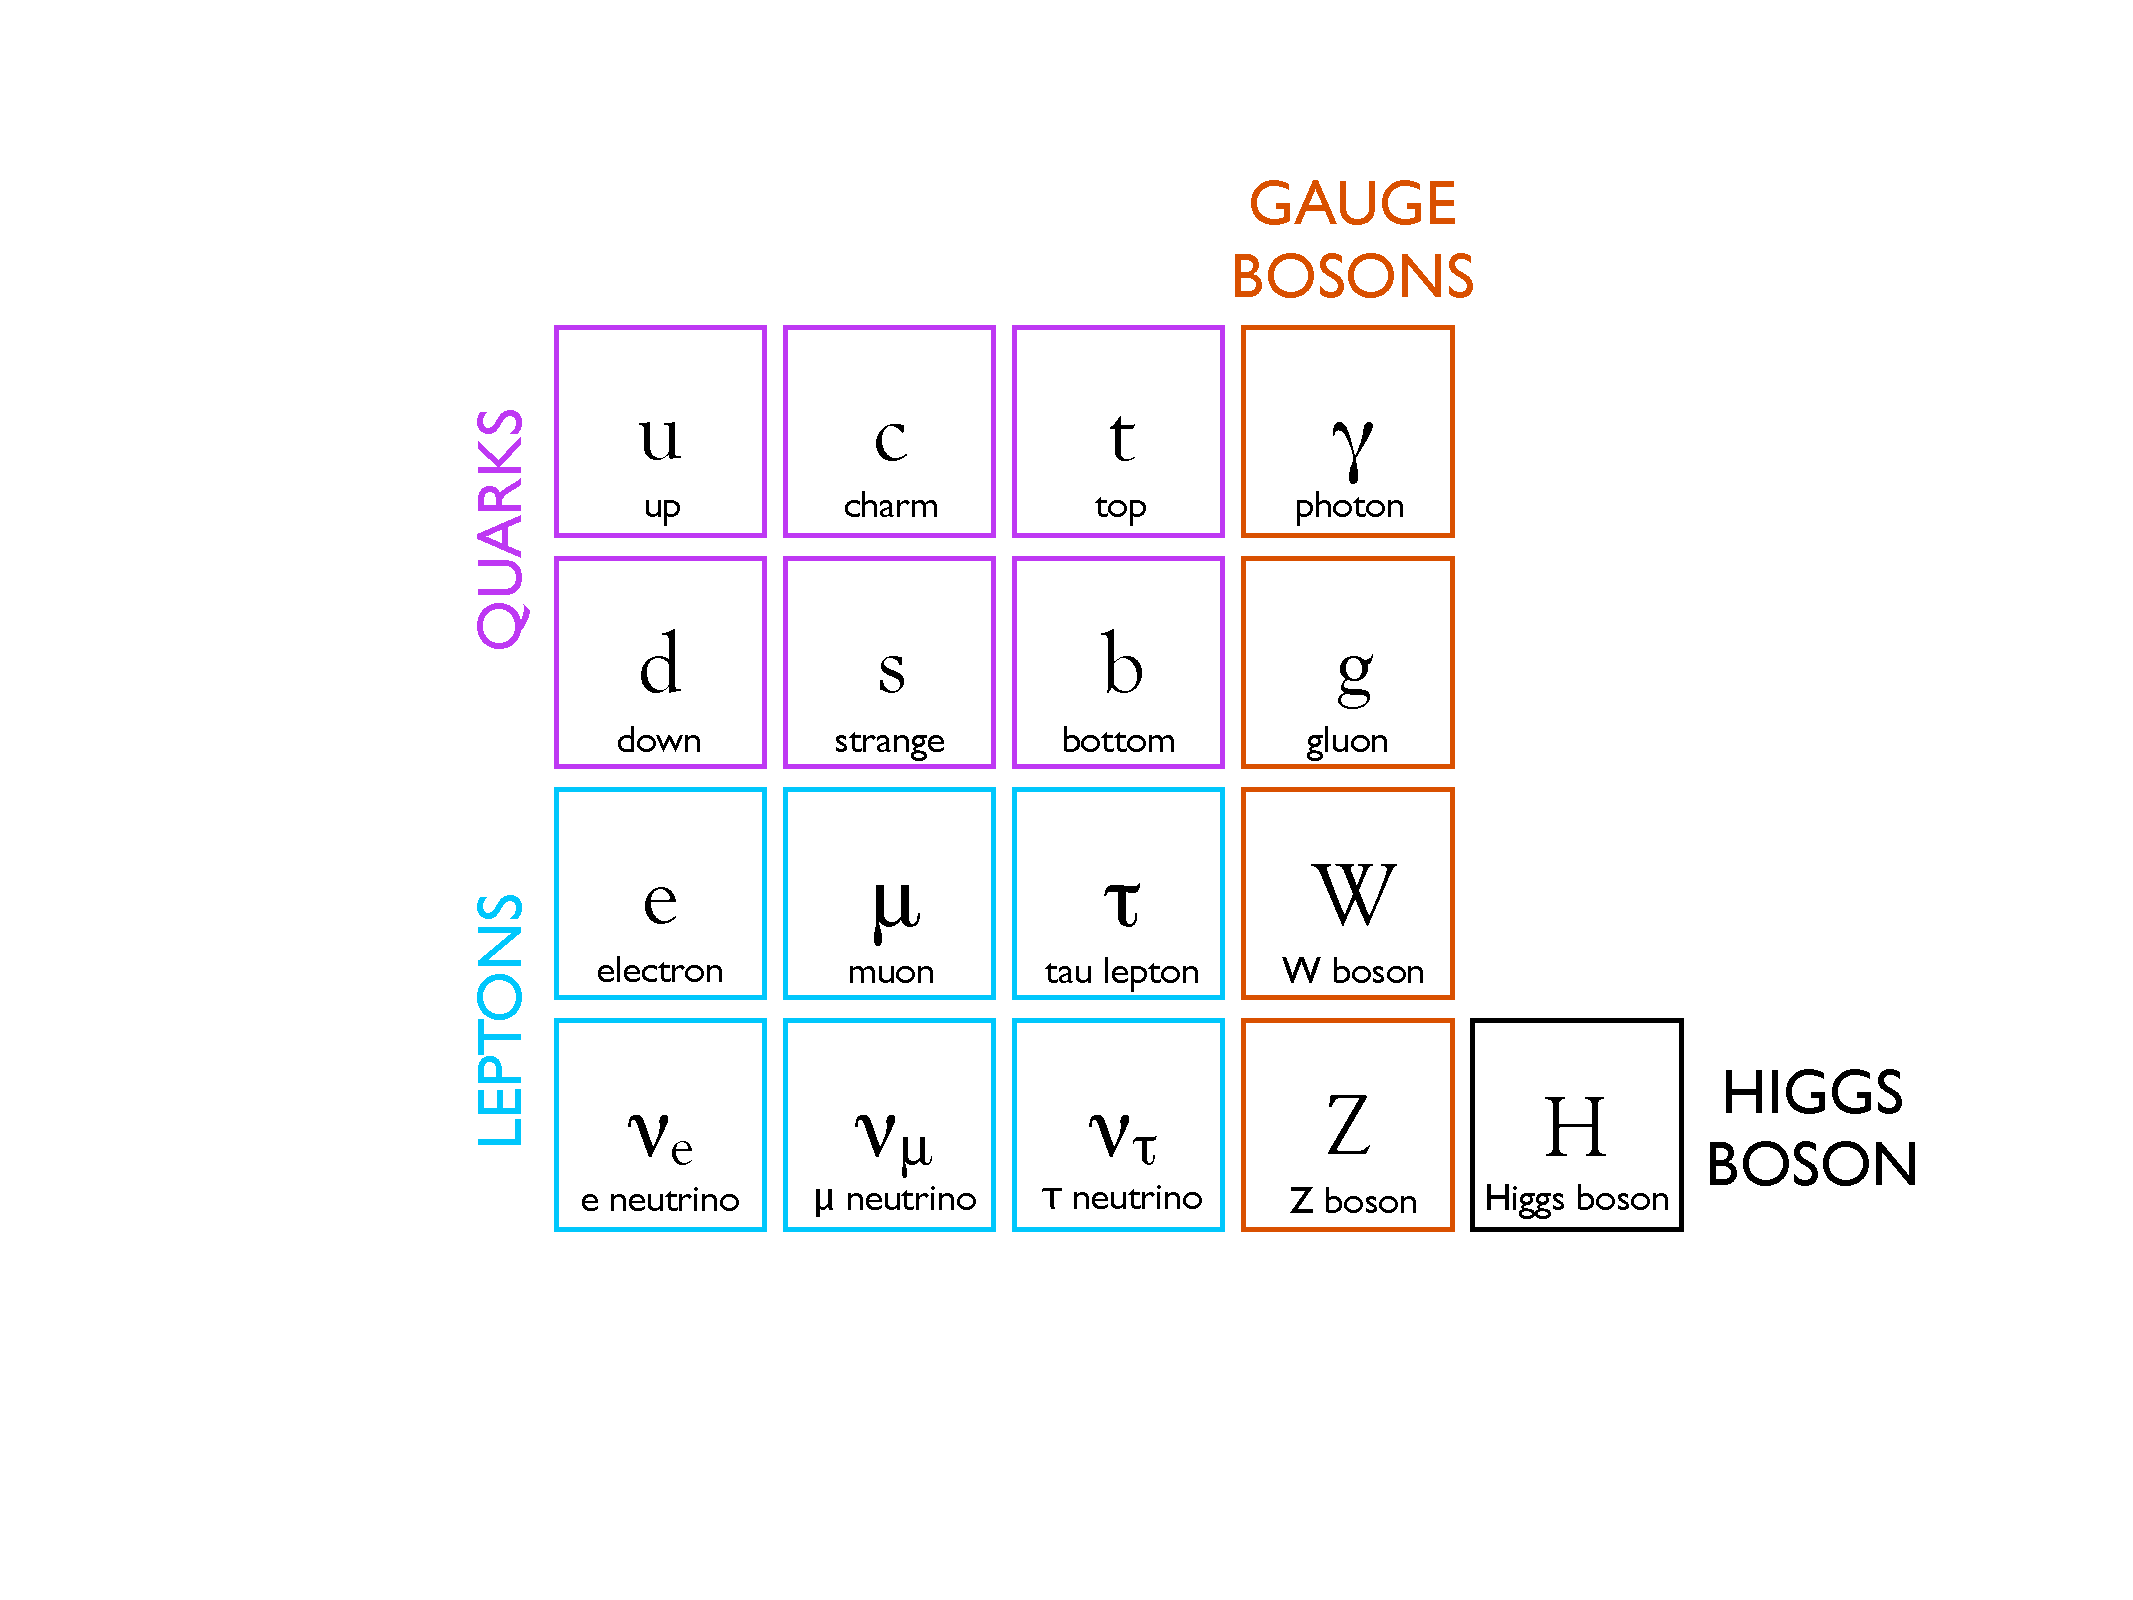
\includegraphics[width=0.6\textwidth]{figures/StandardModelTable}
      \caption{Standard Model particles.}
      \label{fig:StandardModelTable}
   \end{center}
\end{figure}

Leptons and quarks are fermions -- particles with half-integer spin whose dynamics obey the Dirac equation (see Equation~\ref{eq:Dirac}). Leptons fall into three generations called ``flavors", and have electric charge equal to integer multiples of the elementary charge $e =$ 1.6$\cdot$10$^{-19}$ C. The negatively charged leptons are the electron, the muon, and the tau (in increasing order of mass), and each is associated with an extremely light, neutral particle called a neutrino. Quarks have fractional multiples of the elementary electric charge and also possess another quantum property known as ``color" charge, whose implications will be explained shortly. There are three generations of quarks and a total of six different quark flavors (two per generation). For each quark and lepton, there exists an associated antiparticle.

The strong, electromagnetic, and weak interactions occur via the exchange of gauge bosons, which obey Bose-Einstein statistics and have spin 1. Each type of interaction involves the coupling of particles to the gauge field associated with that interaction. The theory describing the strong force is called quantum chromodynamics, or QCD. Quantum electrodynamics (QED) describes the electromagnetic force. At energies above $\mathcal{O}$(100) GeV, the electromagnetic interaction force unifies with the weak force, and the unified force is described by the electroweak theory.

The Standard Model belongs to the symmetry group SU(3)$\times$SU(2)$\times$U(1). The QCD Lagrangian $\mathcal{L}_{QCD}$ obeys the symmetry of the special unitary group SU(3), while the electroweak portion $\mathcal{L}_{EWK}$ obeys SU(2)$\times$U(1) symmetry.

The strong force is mediated by gluons, which are colorless, electrically neutral, and massless; only quarks and gluons, which possess nonzero color charge, can participate in strong interactions. In QCD, the eight generators of the SU(3) group give rise to eight gauge fields $G^{a}_{\mu}$, whose linear combinations correspond to gluons. The conserved quantity in QCD interactions is ``color" charge. An unusual feature of the strong force is that as the momentum transfer of the interaction increases, the strength of the interaction decreases. Thus, for high-energy interactions, the QCD coupling is small enough that perturbation theory can be applied to Feynman diagrams and quarks can be treated like free particles -- a property known as asymptotic freedom. The behaviour of the strong force at low energies, where QCD becomes non-perturbative, is still not well understood; one consequence of the low-energy scale behaviour of the strong force is color confinement, which means that quarks and antiquarks cannot be found free but can only exist in bound states called hadrons. The SU(3) invariance of hadronic wavefunctions restricts the only possible hadronic states to be SU(3) singlets -- i.e., states with a net zero color charge.

The quarks that make up a hadron, the gluons that bind them, and the fleeting quark-antiquark pairs that these gluons produce are collectively known as partons. The probability density for each parton to be found with a fraction $x$ of the total hadronic 4-momentum is described by its parton distribution function (PDF), which is determined by the strong interactions among the various partons in the hadron. In practice, PDFs cannot be calculated from theory alone because of the non-perturbative nature of QCD interactions at low energies; thus, they can only be measured experimentally~\cite{BettiniPhysics}.

Any particle with electric charge can participate in electromagnetic interactions, which are mediated by electrically neutral, massless photons. $W^{\pm}$ or $Z^{0}$ bosons are the carriers of the weak force, which is responsible for such processes as nuclear decays (they will hence be referred to as $W$ and $Z$, dropping the charge superscript unless it is necessary to mention their charges explicitly). $W^{+}$ and $W^{-}$ are one another's antiparticles, while $Z$ and the photon are their own antiparticles. Unlike the gluon and photon, the $W$ and $Z$ bosons are massive.
 
Low-energy weak processes such as beta decays were first described by Fermi via a simple four-point interaction~\cite{0034-4885-42-12-001}. This, however, does not explain the experimental observation of parity violation in weak decays, and the predicted cross-section for weak decays blows up for high-energy processes ($q^2 >$ $\mathcal{O}$(100 GeV)$^2$) in the four-point interaction model. Electroweak theory developed in response to these issues; it predicted that weak interactions occur via parity-violating axial vector currents mediated by massive vector bosons~\cite{PerkinsPhysics}. In electroweak theory, the gauge fields $B_{\mu}$ (from the U(1) group) and \textbf{W}$^1$$_{\mu}$, \textbf{W}$^2$$_{\mu}$, and \textbf{W}$^3$$_{\mu}$ (from the SU(2) group) give rise to the electroweak gauge bosons~\cite{Bednyakov:2007pz}.

However, a problem arises from the fact that the Lagrangian for the electroweak gauge bosons can only be invariant under SU(2)$\times$U(1) transformations if the masses of its gauge bosons are zero. Although the photon is known to be massless, the $W$ and $Z$ bosons are clearly not. A prediction for the mass of the $W$ was first derived from measurements of the lifetime of the muon~\cite{ThomsonPhysics}, and the $W$ and the $Z$ were later both discovered in e$^{+}$e$^{-}$ collisions in the LEP experiment at CERN~\cite{Arnison:1983rp,Arnison:1983mk}.

The massive gauge boson paradox is resolved by the concepts of spontaneous symmetry breaking and the Higgs mechanism~\cite{ThomsonPhysics}. This involves the introduction of a complex scalar field whose vacuum expectation value is not zero but instead one of multiple nonzero minima of the scalar field potential. The choice of one of these vacuum expectation values breaks the symmetry of the scalar potential. This is illustrated in Figure~\ref{fig:higgspotential} for the simplified case of a real scalar potential with two local minima. When the Lagrangian of such a scalar field is expressed in terms of a perturbation of the field about its vacuum expectation value, this results in a mass term for the perturbation that corresponds to a scalar boson called a Goldstone boson.

\begin{figure}
   \begin{center}
      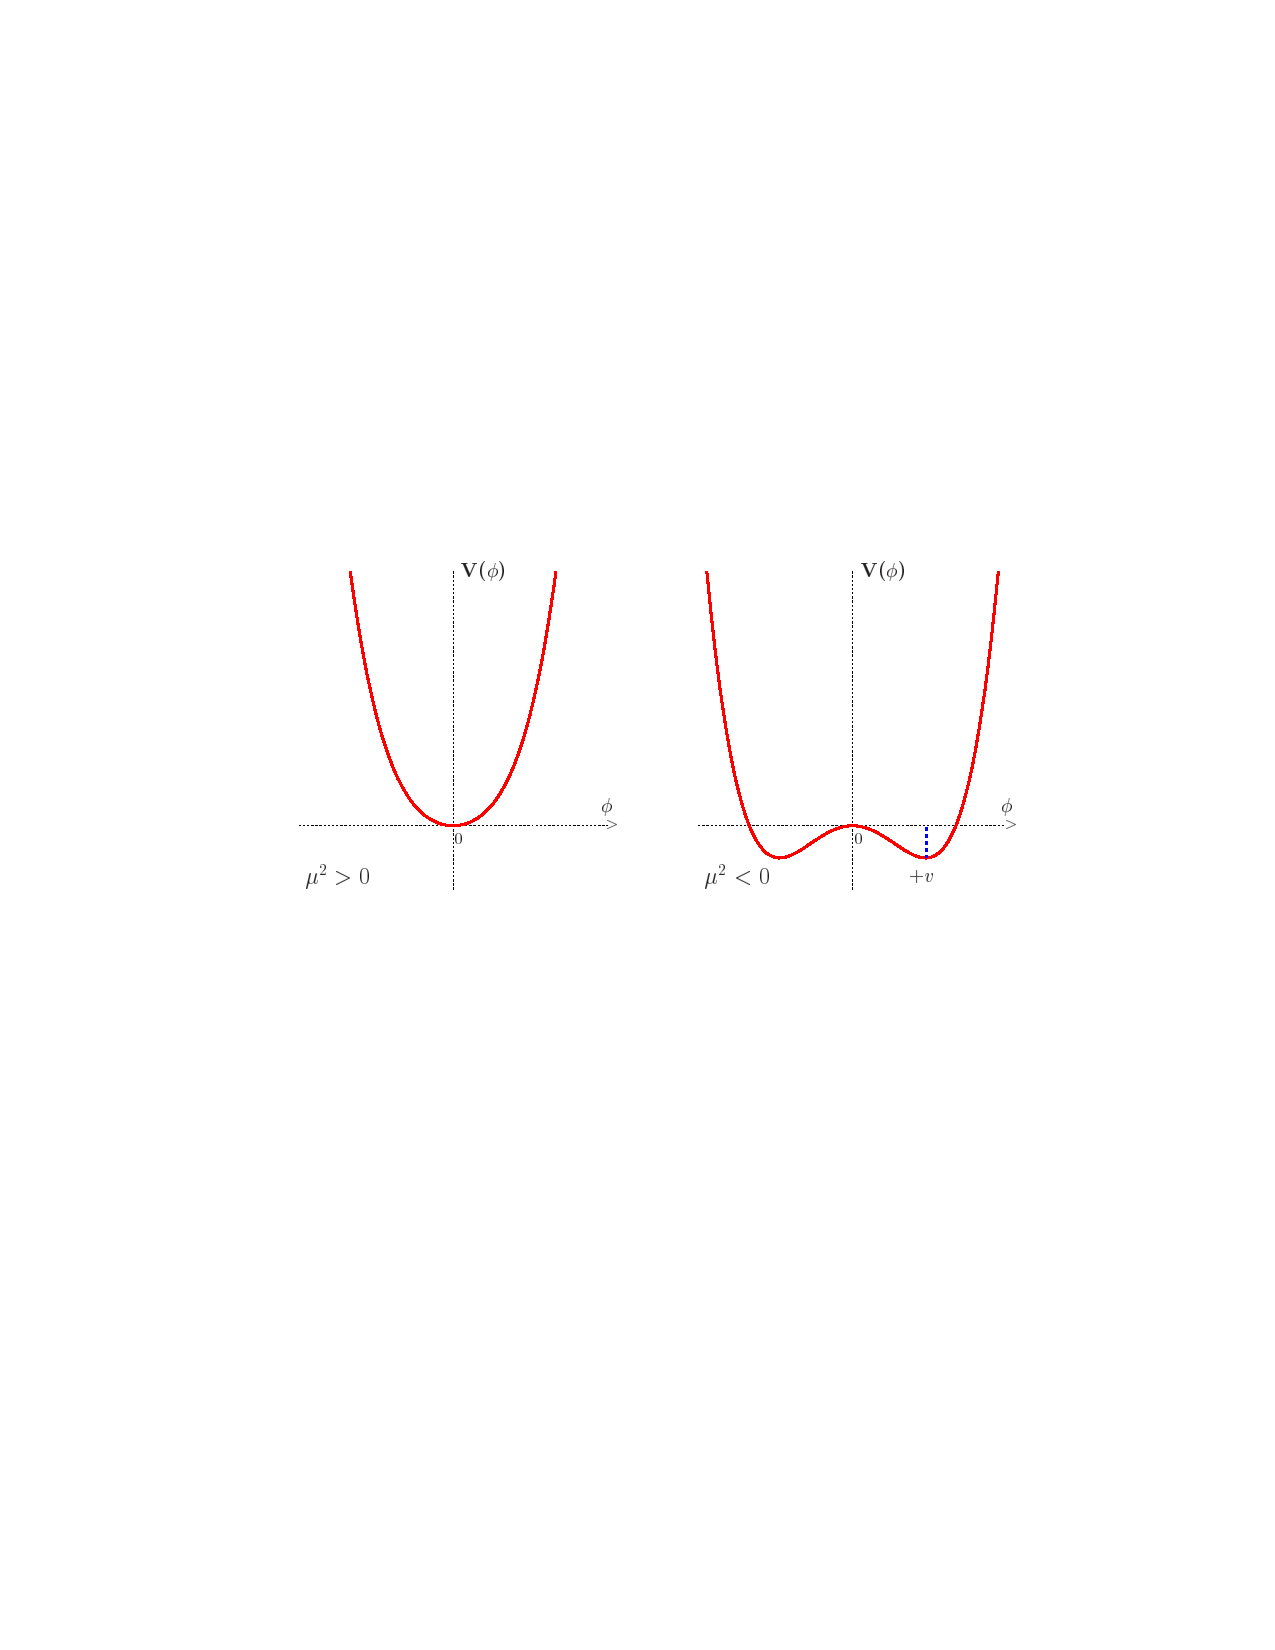
\includegraphics[width=0.6\textwidth]{figures/intro-Higgspotential}
      \caption{Illustration of spontaneous symmetry breaking in the case of a real scalar field $\phi$, with potential V($\phi$) $= \frac{1}{2}\mu^2\phi^2 + \frac{1}{4}\lambda\phi^4$. For $\mu^2 > 0$ (\cmsLeft), the potential has a minimum at zero and thus the vacuum expectation value of the field is zero. For $\mu^2 < 0$ (\cmsRight), the potential has two nonzero minima at $v = \pm\sqrt{-\frac{\mu^2}{\lambda}}$; in nature, the symmetry is broken by the choice of one of these two possible values for the vacuum expectation value of the field. Image copied from~\cite{Djouadi:2005gi}.}
      \label{fig:higgspotential}
   \end{center}
\end{figure}

To complete the picture, the spontaneous symmetry of the scalar field is embedded in the SU(2)$\times$U(1) symmetry, and this results in what is known as the Higgs mechanism. The simplest model requires two complex scalar fields. When the combined Lagrangian of the scalar fields and electroweak gauge fields is expressed as an expansion about the chosen vacuum expectation values of the scalar fields, one ends up with terms quadratic in the $B_{\mu}$, \textbf{W}$^1$$_{\mu}$, \textbf{W}$^2$$_{\mu}$, and \textbf{W}$^3$$_{\mu}$ fields, which are interpreted as mass terms. Via an appropriate gauge transformation, the Goldstone bosons resulting from the symmetry breaking disappear by being absorbed into the longitudinal degree of freedom of the \textbf{W}$^i$$_{\mu}$ fields, and the mixing of the four gauge fields results in the $W^{\pm}$ bosons, which are linear combinations of \textbf{W}$^1$$_{\mu}$ and \textbf{W}$^2$$_{\mu}$, and a $Z$ boson and a photon, both of which are linear combinations of \textbf{W}$^3$$_{\mu}$ and $B_{\mu}$. When this mixing is accounted for in the Lagrangian, the only mass terms that remain are the ones for the $W$ and $Z$ bosons, while the photon is massless. The existence of the Higgs field also generates the masses of the fermions via Yukawa interactions between fermions and the Higgs field in the electroweak Lagrangian.

\begin{figure}
   \begin{center}
      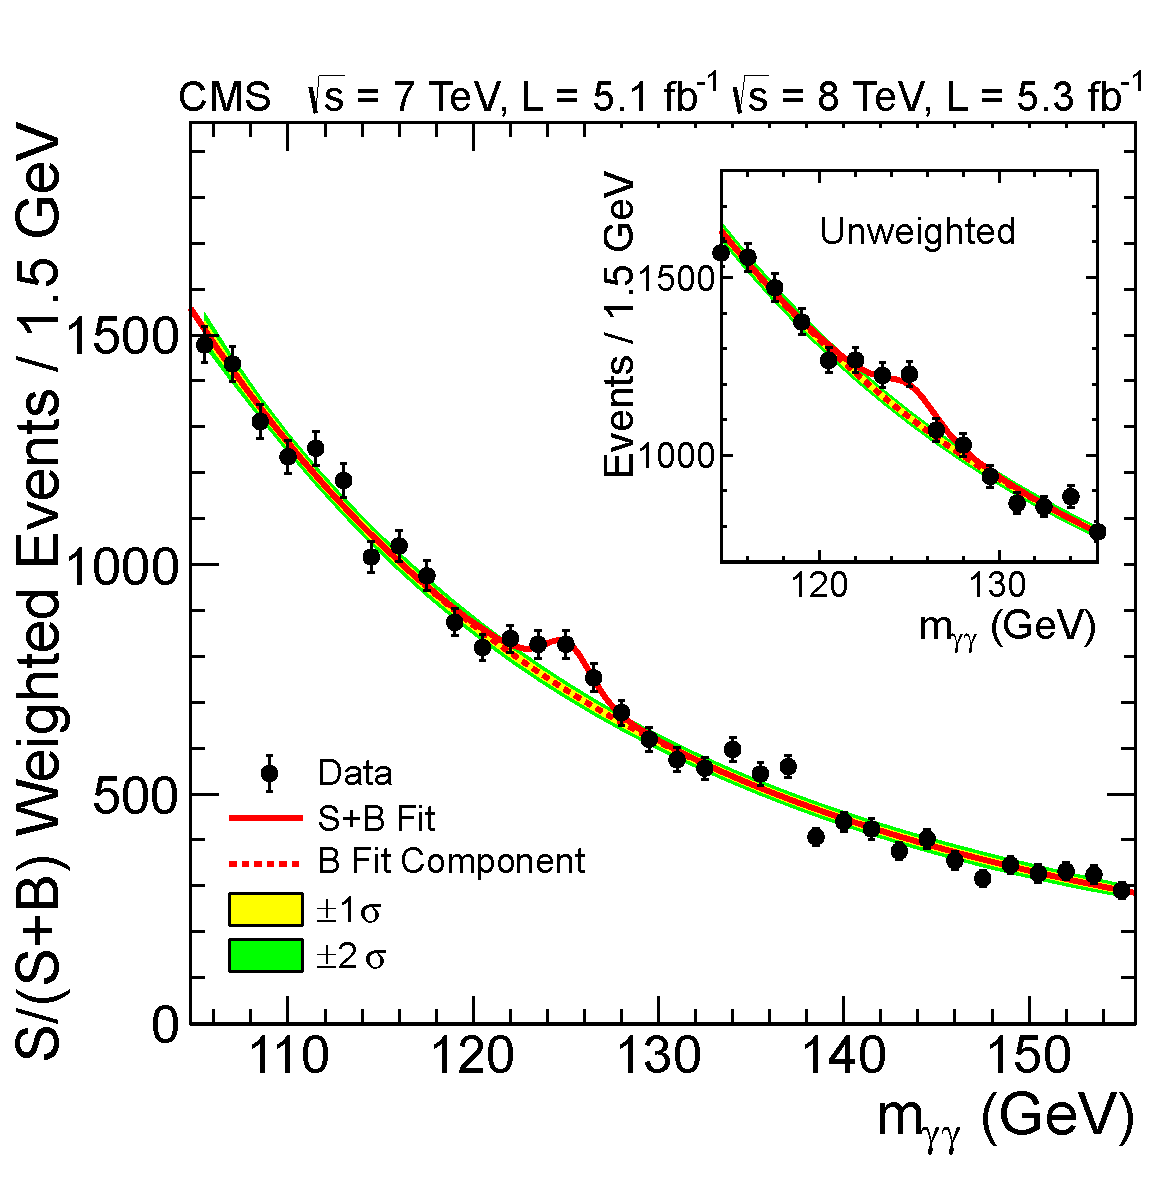
\includegraphics[width=0.45\textwidth]{figures/higgs-resonance-diphoton}
      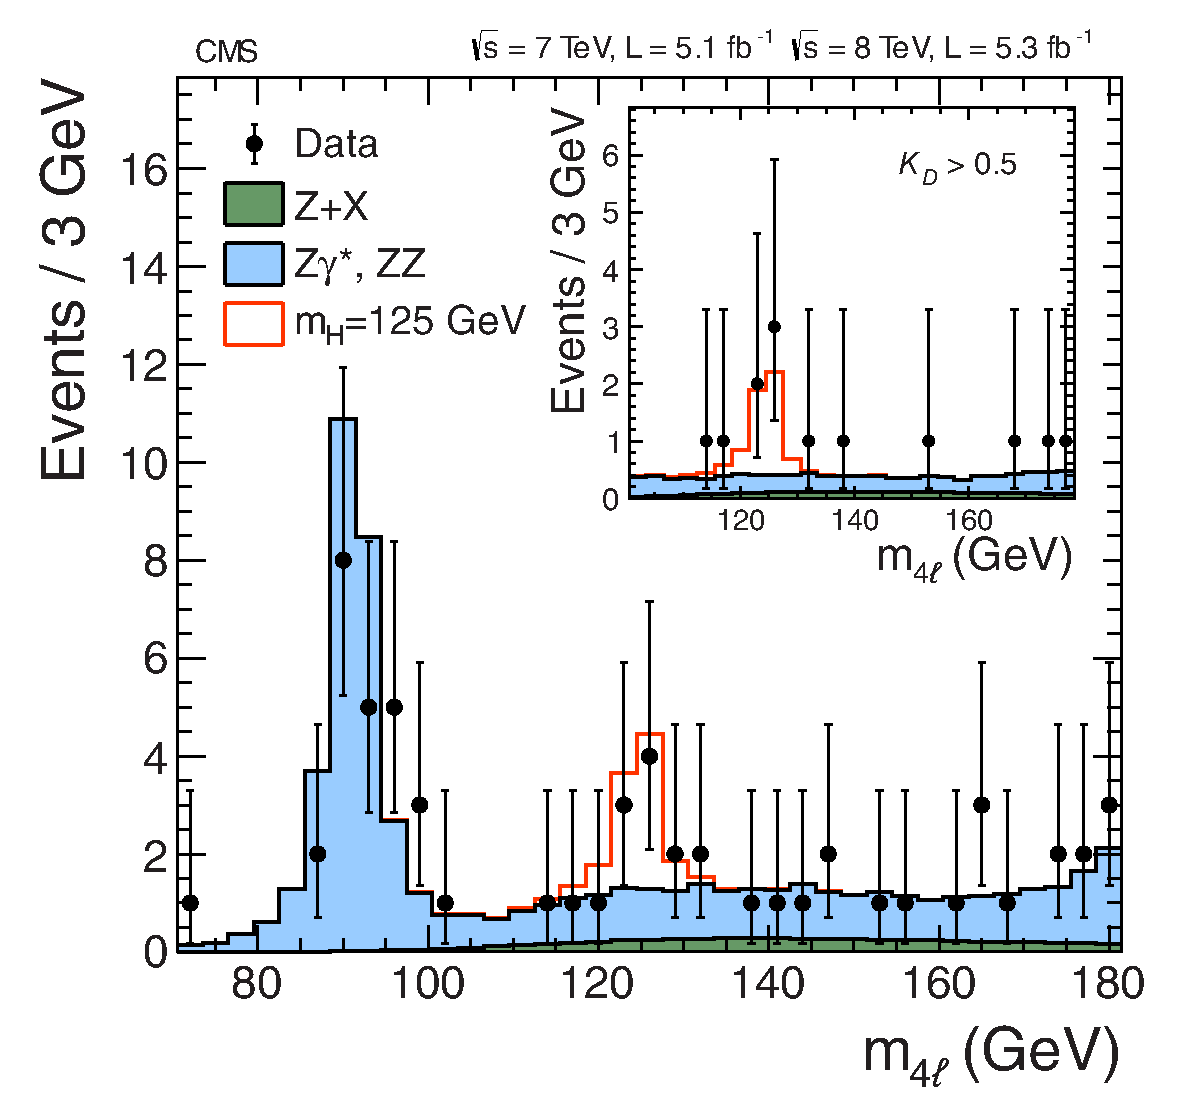
\includegraphics[width=0.47\textwidth]{figures/higgs-resonance-ZZ4l}
      \caption{(\cmsLeft) Observation of the Higgs resonance in the $H\rightarrow\gamma\gamma$ channel at the CMS experiment. The reconstructed diphoton events were grouped into different categories based on different kinematic variables before being combined into the final result; the inset shows the same diphoton mass spectrum, in which the events have not received a weight based on the signal-to-background ratio of their category. (\cmsRight) Observation of the Higgs resonance in the $H\rightarrow ZZ\rightarrow4l$ channel. The inset shows the same spectrum after a further selection step using the probability ratio $K_{D}$ of the signal and background hypotheses. The combined $H\rightarrow\gamma\gamma$ and $H\rightarrow ZZ\rightarrow4l$ channels yield a best-fit Higgs mass of 125 $\pm$0.4 (stat.) $\pm$0.5 (syst.) GeV.~\cite{Chatrchyan:2012ufa}}
      \label{fig:higgs-resonance}
   \end{center}
\end{figure}

Thus, the electroweak theory predicts the existence of a Higgs boson. This is the final particle is represented in Figure~\ref{fig:StandardModelTable}, the only known scalar particle in the Standard Model. The experimental search for this Higgs boson has carried on for decades after its existence was first predicted, and has finally culminated in its discovery at the LHC collider at CERN~\cite{Aad:2012tfa,Chatrchyan:2012ufa} (see Figure~\ref{fig:higgs-resonance}), providing a strong validation for this last major prediction of the Standard Model.

\section{Deficiencies of the Standard Model\label{sec:SMdeficiencies}}

Although the Standard Model has been successful in describing a wide range of experimental results, there is clear evidence that it is not complete. To name a few of its shortcomings~\cite{BettiniPhysics}:

\begin{itemize}
\item \textbf{Gravity: }The four fundamental forces are the strong force, electromagnetism, the weak force, and gravity. The Standard Model accounts for the first three, but the way in which gravity, which is $10^{32}$ times weaker than the weak force, factors into the Standard Model is still unknown.
\item \textbf{Neutrino oscillations: }The Standard Model treats neutrinos as massless particles. However, there is strong experimental evidence to the contrary. The observation of neutrino flavor oscillations, which cannot occur if neutrinos were massless, suggests that the observed electron, muon, and tau neutrino flavors are not in fact mass eigenstates -- rather, the observed neutrino flavor states are superpositions of mass eigenstates. What the mass eigenvalues are and why they are so small, are mysteries that remain to be resolved.
\item \textbf{Dark matter and energy: }Matter constitutes only about 30\% of the total mass-energy density of the universe; the remainder is comprised of ``dark matter" and ``dark energy", but their exact nature is unknown, and their presence is only deduced indirectly from their gravitational effects, since dark matter does not emit or absorb electromagnetic radiation. Thus, it is suspected that dark matter must be made up of some different type of particle not accounted for by the Standard Model.
\item \textbf{Grand unification: }The running coupling constants of the strong, electromagnetic, and weak interactions generally approach one another at increasingly higher energy scales. This suggests that these three fundamental interactions (and perhaps also gravity) might be manifestations of one unified field theory and thus may unify at some high energy scale; some theories predict this scale to be on the order of 10$^{16}$ GeV.
\item \textbf{The hierarchy problem: }The Standard Model predicts that the mass of the Higgs boson receives loop corrections from leptons, quarks, and whatever other particles may couple to the Higgs; Figure~\ref{fig:higgs-loop-corrections} shows two example Feynman diagrams for loop corrections from fermions and scalar particles. 

\begin{figure}[hbtp]
   \begin{center}
      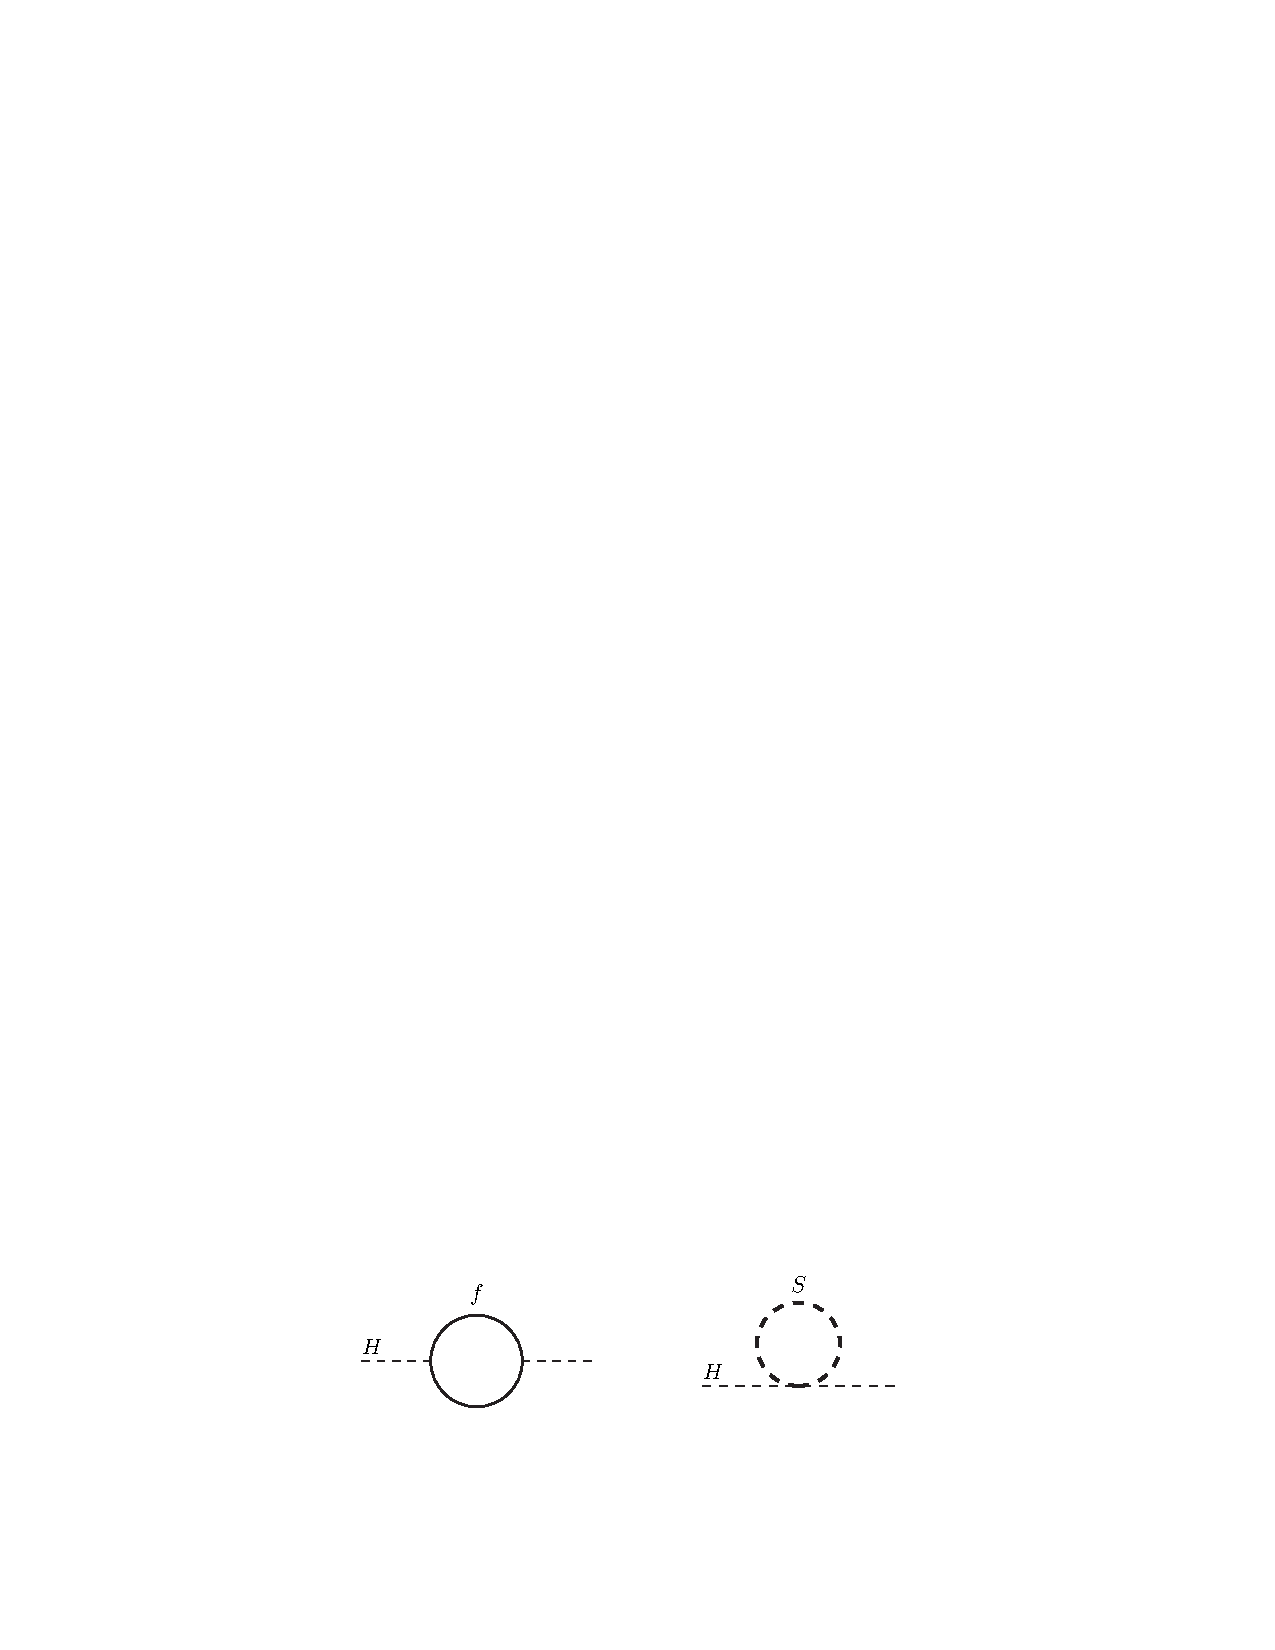
\includegraphics[width=0.6\textwidth]{figures/higgs-loop-corrections}
      \caption{One-loop corrections to the Higgs mass from a fermion $f$ (\cmsLeft) and from a scalar $S$ (\cmsRight)~\cite{Martin:1997ns}.}
      \label{fig:higgs-loop-corrections}
   \end{center}
\end{figure}
To first order, the corrections to the squared Higgs mass from the diagrams in Figure~\ref{fig:higgs-loop-corrections} are:
\begin{equation}
\Delta m_{H}^2 = -\frac{\abs{\lambda_{f}}^2}{8\pi^2}\Lambda_{cutoff}^2 + \frac{\lambda_{S}}{16\pi^2}[\Lambda_{cutoff}^2 - 2m_{S}^2\ln{(\frac{\Lambda_{cutoff}}{m_{S}})}] + \cdots
\label{eq:mH2corr}
\end{equation}
where $\lambda_{f}$ and $\lambda_{S}$ are the Higgs couplings to $f$ and $S$ respectively, and $\Lambda_{cutoff}$ is the cutoff energy scale at which the Standard Model breaks down and new physics takes over. Examples of $\Lambda_{cutoff}$ include the grand unification scale ($\mathcal{O}$(10$^{14}$ GeV)) at which the running couplings of the strong, electromagnetic, and weak forces unify, or the Planck scale ($\mathcal{O}$(10$^{19}$ GeV)) at which gravity becomes significant. Thus, the Higgs mass is expected to receive corrections that are many orders of magnitude larger than its experimentally measured value. The fact that the measured Higgs mass is so much smaller than the predicted corrections is surprising, as it implies the existence of some mechanism, unexplained by the Standard Model, by which these corrections are reduced or cancelled. This constitutes what is known as the hierarchy problem of the Standard Model.
\end{itemize}

These deficiencies indicate that there is physics beyond the Standard Model, and that more elements are needed to provide an accurate description of nature.

\section{Supersymmetry\label{sec:SUSY}}

The theory of supersymmetry provides a means to address the hierarchy problem. This theory posits that there exists a certain symmetry -- called supersymmetry -- that relates fermions to bosons~\cite{Martin:1997ns}. For each fermion, there exists a corresponding bosonic parter particle, and likewise for each boson there exists a fermionic partner; such partner particles are referred to as superpartners. Under a supersymmetric transformation, a fermion turns into its superpartner and vice versa. For each loop correction to the Higgs mass from a Standard Model particle, there would be another loop correction from its supersymmetric partner. Since fermionic loops and bosonic loops have opposite signs, the loop corrections from Standard Model particles are neatly cancelled by loop corrections from their supersymmetric partners.

As supersymmetry predicts the existence of a superpartner for every Standard Model particle, it is of great interest to look for experimental evidence of these superpartners, none of which have yet been observed in nature. The question is where to look, since there is nothing that specifies the masses of supersymmetric particles or the other numerous other free parameters in the theory of supersymmetry. These free parameters must be constrained by experimental measurements.

The masses of supersymmetric particles must be different from the masses of their Standard Model counterparts, otherwise the supersymmetric particles would have been observed already. In order to have this inequality in masses, supersymmetry must be a broken symmetry. There are many models for the mechanism of supersymmetry breaking; but in general, in order to achieve the stabilization of the Higgs mass, the symmetry breaking scale is expected to be on the order of 1-10 TeV~\cite{Aitchison:2005cf}. Since the mass splittings between Standard Model particles and their superpartners are determined by the supersymmetry breaking parameters, the masses of the lightest supersymmetric particles are expected to be around the same scale as well. Thus, if supersymmetric particles exist, it could be possible to discover them in high-energy collider experiments such as the LHC at CERN.

The simplest model incorporating supersymmetry into the Standard Model is the Minimal Supersymmetric Standard Model (MSSM)~\cite{Martin:1997ns}. The details will not be covered here, but the Higgs sector consists of two chiral Higgs supermultiplets $H_u$ and $H_d$, of which the former couples to up-type quarks and the latter couples to down-type quarks and charged leptons. The superpotential $W_{MSSM}$ of the MSSM, which defines the most general non-gauge interactions for the superfields, is:

\begin{equation}
W_{MSSM} = \bar{u}y_{u}QH_{u} - \bar{d}y_{d}QH_{d} - \bar{e}y_{e}LH_{d} + \bar{\mu}H_{u}H_{d}
\label{eq:WMSSM}
\end{equation}

While the MSSM does provide a cancellation of large corrections to the Higgs mass, it comes with deficiencies of its own. One problem, called the $\mu$-problem, stems from the fact that the $\mu$ parameter in Equation~\ref{eq:WMSSM}, which must have the dimension of mass, must be of the order of magnitude of the electroweak scale in order to provide the Higgs doublets with vacuum expectation values on the order of the electroweak scale. However, its magnitude is expected to be more naturally close to the Planck scale, which is significantly larger. Fine-tuning its magnitude to that of the electroweak scale thus seems arbitrary and without theoretical motivation.

Another problem in the MSSM is that the mass of the stop (the supersymmetric partner of the top quark) must be quite large -- on the order of 1-10 TeV -- in order for the lightest CP-even Higgs boson to have a mass greater than 115 GeV without large stop mixing~\cite{Chatrchyan:2012am}. However, such large stop masses would produce large loop corrections to the Higgs mass and quartic coupling, thus reviving the need for fine-tuning. This is referred to as the ``little hierarchy problem"~\cite{Bellazzini:2009ix}.

The $\mu$-problem is avoided in the Next-to-Minimal Supersymmetric Standard Model (NMSSM)~\cite{Maniatis:2009re}, which extends the Higgs sector of the MSSM by a scalar Higgs singlet field S and ultimately predicts a total of seven Higgs bosons -- a pair of charged ones, three neutral scalars, and two neutral pseudoscalars. The NMSSM superpotential is:

\begin{equation}
W_{NMSSM} = W_{MSSM} + \lambda SH_{u}H_{d} + \frac{1}{3}\kappa S^3 + \frac{1}{2}\mu_{s}S^2
\label{eq:WNMSSM}
\end{equation}

The coupling of the singlet field $S$ to the doublet fields naturally generates an effective $\mu$ term via the expectation value of $S$. Thus, $\mu = \lambda$$<S>$, with the desired magnitude near the electroweak scale. The singlet field also provides a mechanism to raise the mass of the lightest CP-even Higgs without requiring large stop masses, thus significantly reducing the little hierarchy problem~\cite{Chatrchyan:2012am,ref1,PhysRevD.39.844} The fact that the NMSSM circumvents these problems, combined with the fact that searches for evidence of the MSSM at the LHC have so far been fruitless, makes the NMSSM of great interest to study. The new physics search presented in this dissertation is a probe into the Higgs sector of the NMSSM.